\documentclass[12pt]{article}
\usepackage{epsfig}
%\usepackage{palatino}
%\parindent=5pt
\parskip=0pt
\hoffset=-1.7cm
\voffset=-40mm
\textwidth=165mm
\textheight=25cm
\def\?{$\spadesuit$}

\begin{document}
\begin{center}
{\Large The Influence of Low-Permeability Material on the L3 Magnet
Field}\\[10mm]

{P. Gl\"assel, University of Heidelberg, 3.12.01}\\[1mm]
\end{center}

The homogeneity of the field in the area of the TPC and TRD is a major
concern for the tracking quality in ALICE. Previous field mappings and
calculations done for the modified magnet doors have given a homogeneity
of the field in the relevant region of about 2.5 mT for the target field
of 0.4 T.

This note presents estimates of the effect of low-$\mu$ material on the
field, primarily in order to check the feasibility of a space frame
structure made of low-$\mu$ stainless steel. The results, however, can be
also used to judge the effects of low-$\mu$ materials in, e.g., detector
structures. 

The stainless steel quality foreseen for the space frame is specified
for a bulk permeability $\mu \approx 1.05$. At welds and cold-formed
spots, however, higher permeability up to $\mu \approx 1.7$ is expected.

A full-fledged 3-d simulation of a space-frame design is way beyond the
scope of this note. Rather, an approach was chosen that looks at the
effects of small pieces of material of different shape and orientation.
The overall effect of a structure can then be derived as a linear
superposition of the pieces, as long as the overall change of the field
is small, which is our condition anyway.

The calculations have been performed with a 2-d program (POISSON) by
adding small elements to an environment with a homogeneous field, tuned
to 0.4 T. In the mode with cylindrical symmetry, small quasi 3-d objects
can be simulated: (i) a small object with similar extension in all 3
dimensions, (ii) a rod of some length along the field direction.  In flat
2-d calculations, (iii) (long) rods perpendicular to the field  can be
simulated. The coordinate convention for the quasi-3d cases 1 and 2 is
shown in Fig.~1, for the 2-d calculations in Fig.~2. The $z$-axis
points in the direction of the (undisturbed) B-field in both cases.

\begin{figure}[bh]
\begin{center}
\parbox{130mm}{
\parbox{60mm}{
\begin{center}
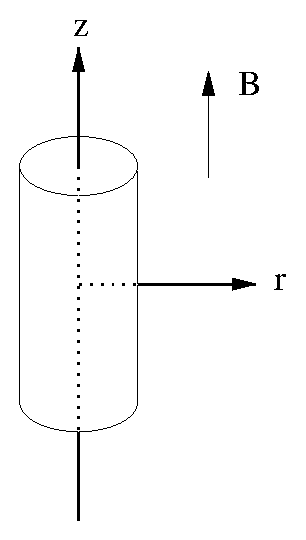
\epsfig{file=coord.eps,width=31.5mm}
\caption{Coordinate system for 3-D calculations}
\end{center}
}
\hfill
\parbox{60mm}{
\begin{center}
\epsfig{file=coordxy.eps,width=48mm}
\caption{Coordinate system for 2-D calculations}
\end{center}
}
}
\end{center}
\end{figure}

  The permeablity is treated as a constant, i.e.\ no saturation effects
occur. In view of the relatively small field ($\mu B < 2$ T) this is
realistic and conservative. 

%The worst possible scenario for magnetic iron, by the way, is
%$mu\approx 5$ at 0.4 T, due to the typical saturation of about 2 T. This
%is a factor 3 worse than the assumptions made here.



\subsubsection*{Some general remarks on the disturbance of homogeneous
fields by magnetic material}

From Maxwell's equations the boundary conditions on %\vec B$ at
interfaces between materials of different permeability $\mu$ are
clear (see e.g. Jackson, Electrodynamics):
\[ \frac{B_{1\perp}}{B_{2\perp}} = 1\quad\quad 
\frac{B_{1\parallel}}{B_{2\parallel}} = \frac{\mu_1}{\mu_2} \]
i.e.\ the normal component is continuous, the parallel component has a
step according to the permeability step. The {\em flux} of $\vec B$ is
continuous (div$B = 0$), equivalent to field lines not ending.
 
This leads to the general phenomenon that the B-field in the magnetic
material tends to be higher by the factor $\mu$. The flux to support the
higher field has to come from the surrounding field. This leads to a
{\em decrease} of the field close to the magnetic material in the
direction lateral to the field.  Before and behind the material, the
higher flux inside the material has to leave the material, with a net
effect of {\em increasing the field} locally. For larger distances from
the material along the field direction, this increase spreads out
laterally and thus decays.  Averaged over an area perpendicular to $z$
and large compared to the size of the material, the {\em mean} field is
unchanged and independent of $z$.


\subsubsection*{1. Small objects with similar extension in all 3
dimensions}

\begin{figure}[h]
\begin{center}
\parbox{150mm}{
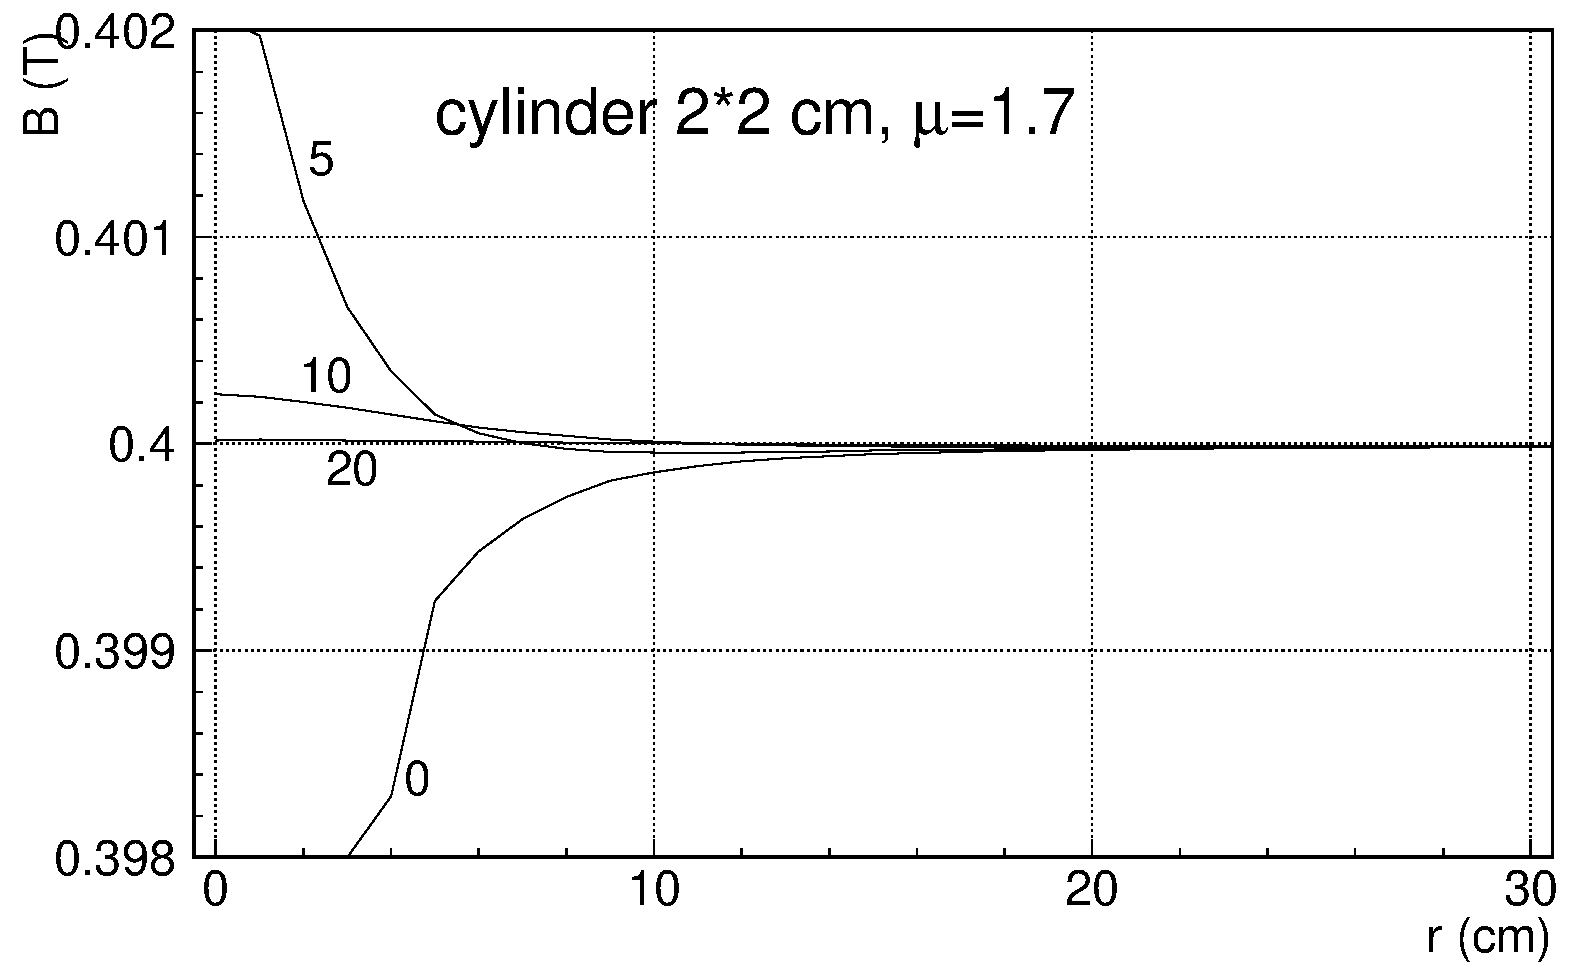
\epsfig{file=l3-2.2c.eps,width=15cm}
\caption{$B_z$ vs $R$ for $z=const$. The numbers label $z$ in cm.}
}
\end{center} 
\end{figure}

Fig.\ 3 shows the z-component of the field near a cylinder of $2\times
2$ cm (diameter$\times$length), $\mu=1.7$, for cuts perpendicular to
the $z$-axis, at different values of $z$. As in all of the following,
$z$ is parallel to the undisturbed, homogeneous field; $r$ (or $x$ in
the 2-d calculations below) counts from the center of the object,
perpendicular to the $z$-axis. The disturbance is below 0.5\% (2 mT)
for distances both in $z$ or $r$ that are about twice the size of the
object and quickly decaying for larger distances. The general
characteristic discussed above is clearly seen: the enhancement inside
the material (off-scale in the figure), the decrease of the field
sideways, the field enhancement close to the axis outside the
material.

%  For an object of larger size \?

\subsubsection*{2. Profiles along the field direction}

For a more realistic simulation of the space frame structure, we look at
a profile along the z-axis. For hollow profiles as forseen for the space
frame, it turns out that the perturbation of the field outside the
profile is well described by a full profile of the outer dimensions with
a constant permeability chosen as the cross-sectional average of the
profile.

\begin{figure}[h]
\begin{center}
\parbox{150mm}{
\epsfig{file=l3-10c.eps,width=15cm}
\caption{$B_z$ vs $R$ for $z=const$. The labels refer to $z$ in
cm; the end of the cylinder is at $z=0$, negative $z$-values cut the
cylinder, positive are beyond the cylinder. (The steps of the field at
material boundaries are not faithfully reproduced due to the
interpolation done by POISSON).}
}
\end{center} 
\end{figure}

\begin{figure}[p]
\begin{center}
\parbox{150mm}{
\epsfig{file=l3-18.10.eps,width=15cm}
\caption{$B_z$ vs $z$ for $x=const$. The labels refer to $x$ in
cm; the profile is centered at $x=z=0$.}
}\\[20mm]
\parbox{150mm}{
\epsfig{file=l3-18.10x.eps,width=15cm}
\caption{$B_z$ vs $x$ for $z=const$. The labels refer to $z$ in
cm; the profile is centered at $x=z=0$. (For the steps see the remark in
Fig.\ 4).}
}
\end{center} 
\end{figure}

Fig.\ 4 shows the case of the outer longitudinal profiles of the space
frame. The dimensions are assumed $200\times 175\times 4$ mm$^2$,
simulated as a full cylinder of 21 cm diameter with $\mu=1.004$.  The
rod extends from $z=0$ to $-\infty$.  For $z<0$ but not too large,
i.e.\ along the rod but close to its end, the field is reduced in the
vicinity of the rod. Farther away from the end of the rod, the reduction
spreads laterally and becomes nearly invisible, in accordance to the
estimates below. Quantitatively, the disturbances are smaller than
$10^{-3}$ everywhere.


For $z<0$, i.e.\ beyond the end of the rod, the field is increased near
the axis of the rod. This increase also spreads and thus decays with the
distance from the rod end. Quantitatively, the perturbation is below the
$10^{-3}$-level about 5 cm away from the rod end.  For the space frame
longitudinal profile, this region near the end of the profiles is
irrelevant for tracking; there might be other cases with longitudinal
material ending inside the tracking volume, however.

 For the space frame structure as a whole, the lateral effect of all
profiles will add up to a reduction of the field along its length. The
reduction can be estimated from the total flux being distributed
according to permeability
\[ B_0  A = \mu B_0 a + B_r (A-a) \] 
with $B_0$ being the undisturbed field, $B_r$ the reduced field
outside the rods, $a$ the total cross section of rods with
permeability $\mu$, $A$ the total cross section of the field. This
leads to

\[ \frac{B_r}{B_0} = \frac{A}{A + (\mu-1)a} \]

For $a = 18\cdot 36$ cm$^2 = 0.065$ m$^2$ and $A= 110$ m$^2$ and
$\mu = 1.05$, $(B_0 - B_r)/B_0 = 3\cdot 10^{-5}$.  This is a comfortably small number, with the main concern 
not the change of the mean field but rather the inhomogeneities of
the same order at both ends of the space frame in the transition region to the
undisturbed field $B_0$.


\subsubsection*{3. Profiles perpendicular to the field}

Here we simulate the case of the outer polygon rings of the space frame.
The profile dimensions are assumed to be $100\times 175\times 3.5$
mm$^3$, in the calculation a full profile $10\times 18$ cm$^2$ is taken
with a permeability $\mu=1.005$. The longer side of the profile is along
the field direction. The calculation is 2-dimensional. The
extension of the rod in the 3rd dimension is infinite, a good
approximation for the closed rings of the space frame.  (For other cases
with rods ending, the results would be valid not too close to the ends.)

Fig.\ 5 shows the field along $z$ for various lateral distances from the
profile. The perturbation is smaller than $10^{-3}$
at about 5 cm from the profile, both in z-direction ($z=10+5$ cm) and
laterally ($x=5+5$ cm).

Fig.\ 6 is the same calculation, but presented in cuts perpendicular to
the $z$-axis.

\newpage


\subsubsection*{The influence of welds}

In welds we expect higher permeability, about $\mu=1.7$. The cross
section of welds at the space frame itself are a few tenths of a cm$^2$.

For simulation, a magnetic rod of 1 cm$^2$ cross section was chosen
(Fig.\ 7). Again, the perturbation is below $10^{-3}$ for distances
larger than about 5 cm from the material in all directions.

\begin{figure}[h]
\begin{center}
\parbox{150mm}{
\epsfig{file=l3-20.1c.eps,width=15cm}
\caption{$B_z$ vs $r$ for $z=const$. The labels refer to $z$ in
cm; the cylinder is centered at $z=0$. (For the steps see the remark in
Fig.\ 4).}
}
\end{center} 
\end{figure}

For the welds in the support beams of the space frame with considerably
larger cross section (up to about 10 cm$^2$), no perturbation is expected
as they run along the total length of the magnet and even join to the
magnet yoke.

 

\subsubsection*{Conclusions}

The effect of the bulk material of a space frame made of material with
$\mu =1.05$ is negligible, with a reduction of the avagerage field and
large-scale inhomogeneities of order $< 3\cdot 10^{-5}$.  The weld areas
with higher $\mu$ up to 1.7 are harmless is the cross section is not
larger than order cm$^2$.  If their total volume is not more than a few
\% of the material, their overall effect is also negligible.  The local
distortions of the field are less than about $10^{-3}$ at a distance of
order 5 cm from the structure.

\end{document}